\documentclass[12pt, letterpaper]{article}

\title{Final Project Report: SMASH}
\author{Nathan Roach, Patricia Walchessen, Charlie Wang, and Yue Zhang}
\date{December 8, 2017}

\usepackage[utf8]{inputenc}
\usepackage{blindtext}
\usepackage{cite}
\usepackage{color}
\usepackage{comment}
\usepackage{csquotes}
\usepackage{graphicx}
\usepackage[numbers]{natbib}
\usepackage{wrapfig}
\usepackage{placeins}

\setlength{\parindent}{4em}
\setlength{\parskip}{1em}

\begin{document}

\maketitle
% ----------------------------------------------------------------------------------------------------------------------------
% Abstract
% ----------------------------------------------------------------------------------------------------------------------------
\begin{abstract}
	[1 paragraph] \color{red} TO DO \color{black} Final Project Abstract
\end{abstract}

% ----------------------------------------------------------------------------------------------------------------------------
% Introduction
% ----------------------------------------------------------------------------------------------------------------------------
\section{Introduction}
An intriguing and common problem that arises in computation is efficiently determining similarities between high-dimensional data. The problem reaches into the far corners of computation, including machine learning and kernels. In bioinformatics, the problem takes the form of determining the similarity between both close and disparate long genomic sequences. Solving the challenge of comparing long genomic sequences would aid in evaluating evolutionary relationships, determining the organismal source of sequencing data, and comparing metagenomic data. \\ \\
One class of algorithms that could solve this problem is Locality-Sensitive Hashing (LSH) algorithms. LSH algorithms reduce data dimensionality and bin inputs such that similar data sets are grouped together with high probability. They solve the problem of approximate or exact Near Neighbor Search. In recent years, LSH algorithms have offered solutions to problems such as near-duplicate detection, genome-wide association, and both image and audio similarity identification. There are two prevalent LSH algorithms: MinHash and SimHash. \\ \\
MinHash computes the differences between two genomic sequences through the estimation of a Jaccard Index, a ratio of the shared identity between the sets. SimHash, on the other hand, estimates the cosine similarity by weighting the frequency of the bits, compiling them into vectors and evaluating similarity by the distance between the vectors. The application of MinHash across multiple fields of research has been explored, including in the field of computational genomics. The application of SimHash, on the other hand, has been more limited. After additional research, we found no reference of the exploration of SimHash or any other LSH in the comparison of genomic sequences. Thus, we pursued a research project on the competing LSH, SimHash. This project is a pioneering foray of SimHash into the field of computational genomics. \\ \\
This project encompasses the exploration of both MinHash and SimHash with respect to the resemblance between genomes. The approach started with the exploration of MinHash, as the research already exists to better further the understanding and knowledge of the field. Next, SimHash was applied to the field. From the ensuing results, SMASH was developed to address a major shortcoming within SimHash.

% ----------------------------------------------------------------------------------------------------------------------------
% Prior Work
% ----------------------------------------------------------------------------------------------------------------------------
\section{Prior Work}
The main contribution of LSH into the computational genomics field was an implementation of MinHash to analyze the resemblance between genomes and metagenomes by Ondov et al. in 2016.\cite{MinHash} They altered the MinHash algorithm to include pairwise mutation distance, or Mash distance, which estimates the rate of sequence mutation under a simple evolutionary model. Their modifications allowed Mash to efficiently cluster and search massive sequence collections. Mash, as they call their implementation, has two main components: \textit{sketch} and \textit{dist}. The \textit{sketch} function creates MinHash sketches from a sequence or a collection of sequences. \textit{Dist} compares two sketches and returns an estimate of the Jaccard index (ratio of the shared identity between sets), a P value, and the Mash distance.
\FloatBarrier
\begin{figure}[h!]
	\centering
	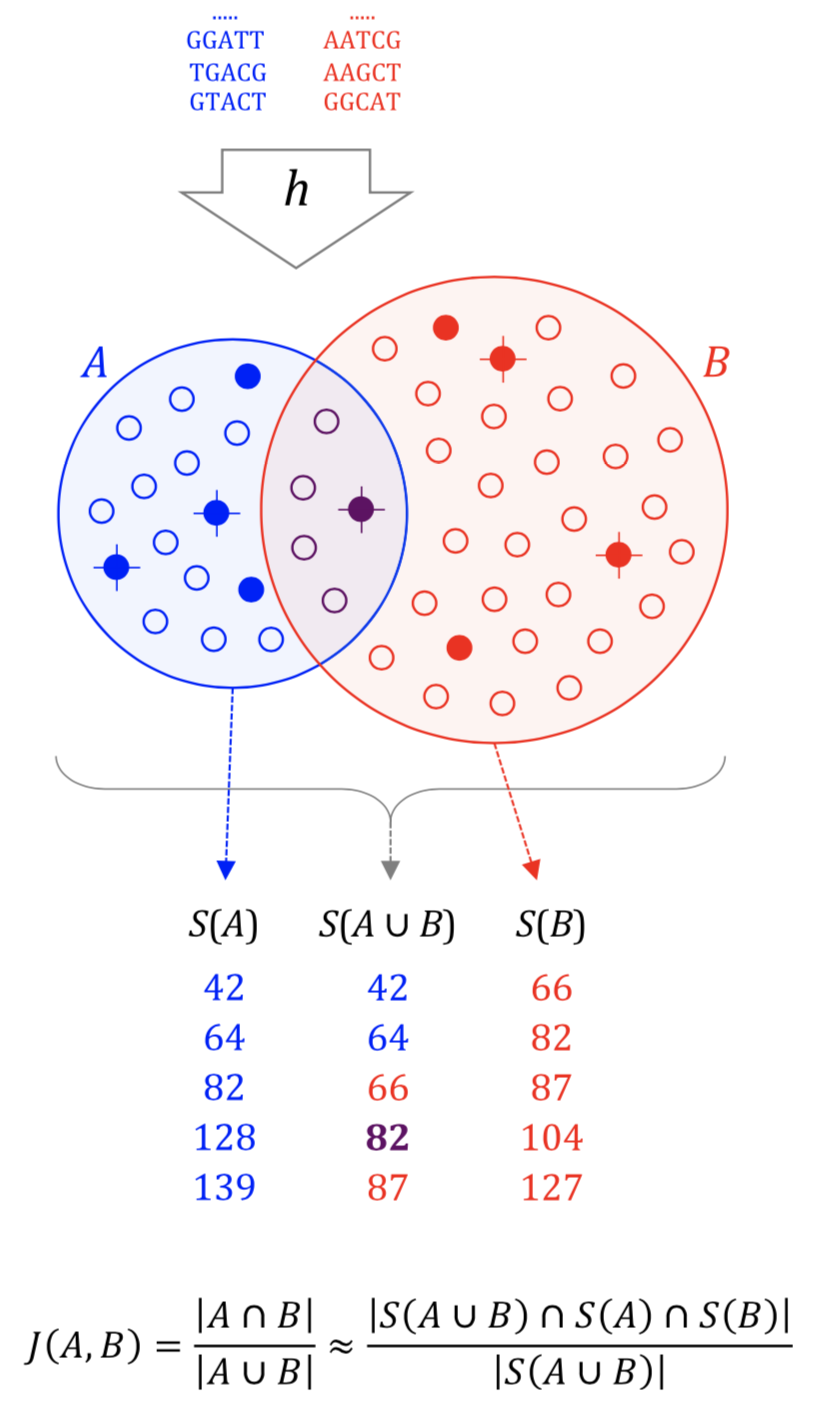
\includegraphics[width=0.5\textwidth]{Mash_description.png}
	\caption{Description of MinHash: First, the sequences are divided into their constituent k-mers. Each k-mer is then passed through a hash function to obtain a 32- or 64-bit hash. The Jaccard index is ratio of shared hashes between A and B over all distinct hashes in A and B. This index can be approximated by considering a smaller subset of A and B. MinHash sketches S(A) and S(B) of size 5 are shown for A and B, comprising the five smallest hash values. The Jaccard Index is determined by dividing the similarity between S(A) and S(B) by the distinct values in S(A) and S(B).}
\end{figure}
\FloatBarrier
Two important parameters within Mash are sketch and k-mer sizes. The larger the sketch size, the better accuracy of the Mash estimates, particularly for divergent genomes. However, the downside is the increase in space and time required for computing the distances. Similarly, the determination of k-mer size alters sensitivity and specificity. Smaller values of k-mer size are more sensitive for divergent genomes, but lose specificity for large genomes due to k-mer collisions. Larger values of k-mer size lose sensitivity. Thus, choosing the smallest k-mer size that reduces chance collisions is important and the optimal k-mer size will change depending on the divergence of the genomes. To maximize sensitivity and specificity, Mash uses a default k-mer size of 21 and a sketch size of 1,000. According to preliminary research by Ondov et al., Mash can be used to cluster whole genomes, identify the genome in real-time  from assemblies or reads, and cluster massive metagenomic databases. \\ \\
Mash has been used to cluster all of the NCBI RefSeq Release 70, totaling 54,118 organisms and 618 Gbp of genomic sequence. The resulting sketches yielded a compression factor of more than 7000-fold versus the uncompressed FASTA (93 MB vs. 674 GB) and only took 33 CPU hours of a typical computer in 2016.\cite{MinHash} Additionally, adding a genome to the database took approximately 0.9 CPU seconds per 5 MB genome. However, fast and space-efficient only works if results are valid. A comparison of Mash distance and ANI, a  measure of genetic similarity, among a subset of 500 E. coli genomes, found Mash distances correlate well with ANI. For a sketch size of 1,000 and k-mer size of 21, Mash approximates 1 - ANI with a root-mean-square error of 0.00274. Thus, Mash enables scalable, whole-genome clustering. \\ \\
With a pre-computed sketch database, Mash is able to identify isolated genomes from both assemblies within a few seconds and identify the Lowest Common Ancestor (LCA) from raw sequencing reads within a couple of minutes. Additional work is needed so Mash can be used to discern genome identity from raw sequencing reads, possibly by filtering out low frequency k-mers or increasing the sketch size. \\ \\
Another important accomplishment is in regard to overcoming the challenge of computing large-scale metagenomic comparison, a problem that more and more are facing. Mash has been shown to cluster metagenomic datasets in a fraction of the time other metagenomic comparison tools use. DSM, which uses an exact Jaccard Index, and COMMET, which attempts to identify a set of similar reads between two samples using Bloom filters, are both metagenomic comparison tools commonly used today. In a comparison between COMMET and Mash on a pool of Global Ocean Survey (GOS) data, Mash was over ten times faster than COMMET and correctly identified clusters from the original GOS study. Thus, Mash provided a time efficient way to analyze and cluster large-scale metagenomic data. Mash enables the comparison and clustering of whole genomes and metagenomes on a massive scale. \\ \\
The original paper on SimHash laid out the intuition behind SimHash, allowing a better theoretical knowledge in the quest to develop SMASH.\cite{simhash} SimHash is an algorithm that first sums up the number of hits per tag used and then runs a hash function on the sum table to convert it to a key. The key is then compared to other keys using the sum of the absolute values of the di↵erences between their entries. \\ \\
In 2014, Shrivastava et al. compared MinHash and SimHash on binary data and determined MinHash was consistently better than SimHash irregardless of the dataset or the number of hash functions used \cite{SimvsMin}. When compared in a worst case scenario as well as in an idealized scenario, Shrivastava et al. stated that MinHash outperformed SimHash, which held up in a number of tests on actual data. For binary data, Shrivastava et al. proved theoretically that MinHash is a sensitive family of hash functions for cosine similarity. Although the results for binary data suggest that MinHash is a better LSH algorithm, no tests have yet been done on how SimHash realistically performs on genomic data, an area that is yet to be explored.

% ----------------------------------------------------------------------------------------------------------------------------
% Methods and Software
% ----------------------------------------------------------------------------------------------------------------------------
\section{Research Methods and Software}

\subsection{Exploration with MinHash}

We explored the algorithm and libraries of MinHash to better understand its properties, better understand how MinHash performs and works, and confirm we are able to achieve the results of the MASH paper.

\subsubsection{Dataset}
The data we ran the MinHash library on was downloaded from the NCBI reference database on December 7, 2017. To determine how MinHash performs on similar data, we downloaded 300+ complete \textit{E. coli} genomes, which were then compared between each other. For development of the phylogenetic tree, we dewnloaded the reference genomes of the following species: \textit{Callithrix jacchus}, \textit{Carlito syrichta}, \textit{Chlorocebus sabaeus}, \textit{Gorilla gorilla gorilla}, \textit{Homo sapiens}, \textit{Macaca fascicularis}, \textit{Macaca mulatta}, \textit{Microcebus murinus}, \textit{Nasalis larvatus}, \textit{Nomascus leucogenys}, \textit{Otolemur garnettii}, \textit{Pan paniscus}, \textit{Pan troglodytes}, \textit{Papio anubis}, \textit{Pongo abelii}, \textit{Rhinopithecus roxellana}, and \textit{Saimiri boliviensis boliviensis}.

\subsubsection{Method}
We used a Python implementation of Mash called SourMash, which was developed by Titus Brown and Luiz Irber from UC Davis and is available as an open-source software \cite{GitHub-SourMash}.

\subsection{Exploration with SimHash}
\subsubsection{Dataset}
The data we tested on encompassed many of the 300+ \textit{E. coli} genomes as well as multiple diverse yeast genomes. For the purpose of the discussion in this section, we will talk about the methods developed based on empirical testing on a dataset consisting of 1 \textit{E. coli} genome and 2 yeast genomes named \textit{S. cerevisiae} and \textit{S. pombe}.

\subsubsection{Method}
To fully explore the application of SimHash in the genomics field, we commenced by surveying the existing SimHash literature and implementations. Next, we looked for existing SimHash libraries, many of which were designed for analyzing websites or texts of English words, and compiled the most reputable ones. From there, we selected two based on their reputation and fork numbers for us to base our code on and to adapt into the genomic field to explore SimHash more extensively. The first is Python-based \cite{python-simhash} and the second is Go-based \cite{go-simhash}.

\subsubsection{Python-based SimHash}
Upon surveying the existing code in the Python-based SimHash, we found there were hard-coded values in the library, such as k-mer or shingle sizes of 4. We thus took account of hard-coded values, then created our own SimHash class based on the Python-based SimHash. The goal with our SimHash class is to enable it to fundamentally accept genomic data and build shingles based on genomic data. Of note was its reliance on using MD5 to hash the keys, then performed the operations of SimHash and the hamming distance on the MD5 hashes. The hashes were also only 32 bit. In all, we coded a more flexible Python-based SimHash library for running our tests of SimHash on genomic data.

\subsubsection{Go-based SimHash}
Our design and coding of the Go-based SimHash was similar to the Python-based SimHash. By basing our code on the Go library, we made a fundamental modification to accept genomic data. A special particularity with the unmodified Go-based SimHash library is that although the library has a method for making shingles of words, it does not appear to be used. Also, the unmodified Go-based SimHash library assumes the input is string of English words that could or could not be encoded in Unicode. Thus, we made fundamental modifications to the feature construction in the Go-based SimHash library to accept genomic data. Some of the modifications included building the features based on whether it is a substring of lowercase bases or uppercase bases, or building the features based on a k-mer size of 15. We continued with the use of 64 bit hashes in Go.

\subsubsection{Evolution of our Research}
With both our Python-based SimHash and Go-based SimHash code, we fed in genomic data to test how the core SimHash algorithm performs. Recall that the genomic data consisted of one strain of E. coli, approximately 4.5 million bases, and two yeast strands, approximately 12 million bases each. After running the SimHash algorithm in each respective language and observing the output of the distance between the genomic data, we found the results were inaccurate above a certain k-mer length and not always consistent for data below the threshold. \\ \\
In a comparison between one of the yeast strands and the E. coli the SimHash algorithm was able to distinguish that they were quite different. However, the SimHash algorithm outputted the difference between the other yeast strand and E. coli vs. the difference between both of the yeast strands was approximately equivalent. Fundamentally, from the sole fact of differences in the length of the genome, the result showed that SimHash was losing resolution. \\ \\
We first thought these results might be due to how the Python-based SimHash was using the MD5 hash and was implementing SimHash. However, by bringing in the Go-based SimHash, which does not use a MD5 hash but the raw bit values and computes the SimHash fingerprint based on a bit by bit operation with weighting, both returned similarly lackluster results showing the implementation of SimHash is not likely the factor.  \\ \\
We next explored whether the results were because of how we inputted the genomic data. We explored different k-mer sizes and also decided to normalize the data by converting all the bases to lowercase letters. However, even attempts at standardizing the genomic data or exploration of different shingling sizes did not alter the lackluster results from SimHash. Thus, we concluded it is likely due to how the SimHash algorithm is designed. \\ \\
We further reviewed the literature and discovered that SimHash was primarily designed for finding small discrepancies between websites. Thus, the design principle of SimHash is to have a good high resolution of small amount of changes. Thus, it can be implied that SimHash is unable to accurately handle large differences or hamming distances. With a hamming distance of over 20, SimHash started losing resolution of the distance between the hashes. Thus, we needed to find a way to make up for the loss of resolution.


\subsection{SMASH}
Thus came the development of original research based on what we learned and observed from MinHash and SimHash. Seeing how the existing SimHash algorithm was losing resolution when the Hamming distance was too great, we went back to the drawing board and examined each part of the SimHash algorithm closely. From the examination and with additional brainstorming, we came up with SMASH, which is designed to primarily address the shortcoming of resolution loss with SimHash.

\subsubsection{Design}
One of the major loss of resolution with SimHash was with the following: when a E. coli genome with some 4.5 million bases is compared to one of the yeast genomes with 12 million bases, SimHash outputs that it is about the same hamming distance apart as another comparison, which is instead between to two yeast genomes and which both of which have about 12 million bases. Thus, we sought to address the loss of frequency in the resolution.  \\ \\
First, we observed that the basic property of the LSHs were the consensus to find a way to build a feature structure out of the dataset. In our case, we decided to build our feature structure based on frequency. The way this is handled is that for each of the genome file that is inputted, we parse it such that it becomes one complete contiguous string. Next, we chop it up into the respective k-mers. An important thing to note is that the size of the k-mer needs to be specified beforehand, and thus we test for the optimal k-mer size and describe it in the Results section. The frequency is based on how frequently the k-mers show up in the respective genome files. \\ \\
Based on the order of the feature structure, we then construct vectors consisting of the frequency of the k-mers. This is then fed into the cosine similarity function, which is used in SimHash, to compute the cosine similarity. Notice that a fundamental difference between SimHash and SMASH is that while SimHash focuses on computing a weighting of frequency of bits, SMASH is instead focusing on computing a weighting of frequency of k-mers. For a finer look into what SMASH does, the pseudocode for the algorithm is accompanied in the next section.

\subsubsection{Algorithm}
\begin{verbatim}
file1, file2 = input 2 genome files 
k = k-mer size

for each file:
    parse and format into one contiguous string

for each file:
    file1_kmers, file2_kmers = divide up file into k-mers

file1_count = dict()
file2_count = dict()

for each kmer in file1_kmers:
    file1_count[kmer] += 1

for each kmer in file2_kmers:
    file2_count[kmer] += 2

for subset of observed k-mers in file_1:
    vector1 = vector of kmer counts from file1_count

for subset of observed k-mers in file_2:
    vector2 = vector of kmer counts from file2_count

similarity_distance = 1 - cosine(vector1, vector2)
\end{verbatim}

\subsubsection{Further Development}
To speed up the counting of k-mers, we explored the use of bloom filter though a Python library called Jellyfish \cite{Jellyfish}. We saw a decrease in needed computation time to achieve our the results highlighted by the above algorithm.

% ---------------------------------------------------------------------------------------------------------------------------
% Results
% ---------------------------------------------------------------------------------------------------------------------------
\section{Results}

\subsection{MinHash}
In our exploration of MinHash we compared whole genomes of varying similarity to both replicate the data in the paper by Ondov et al. and evaluate the MinHash algorithm as a whole. To replicate the results of Ondov et al., we ran MinHash on a set of primate genomes to create a pylogenic tree. This tree was then compared to the trees obtained by the UCSC genome browser and Ondov et al. to determine if MinHash was performing correctly.\ref{fig:Primate Tree} The resulting phylogenetic tree was slightly different from the reference trees. In our result, the Philippine tarsier was closer to the Northern greater galago and Gray mouse lemur. Additionally, we obtained the result that Chimpanzees are closer to Humans than to Bonobos, a result echoed by Ondov et al.'s implementation of MinHash. \\ \\
\begin{figure}[h]
    \centering
    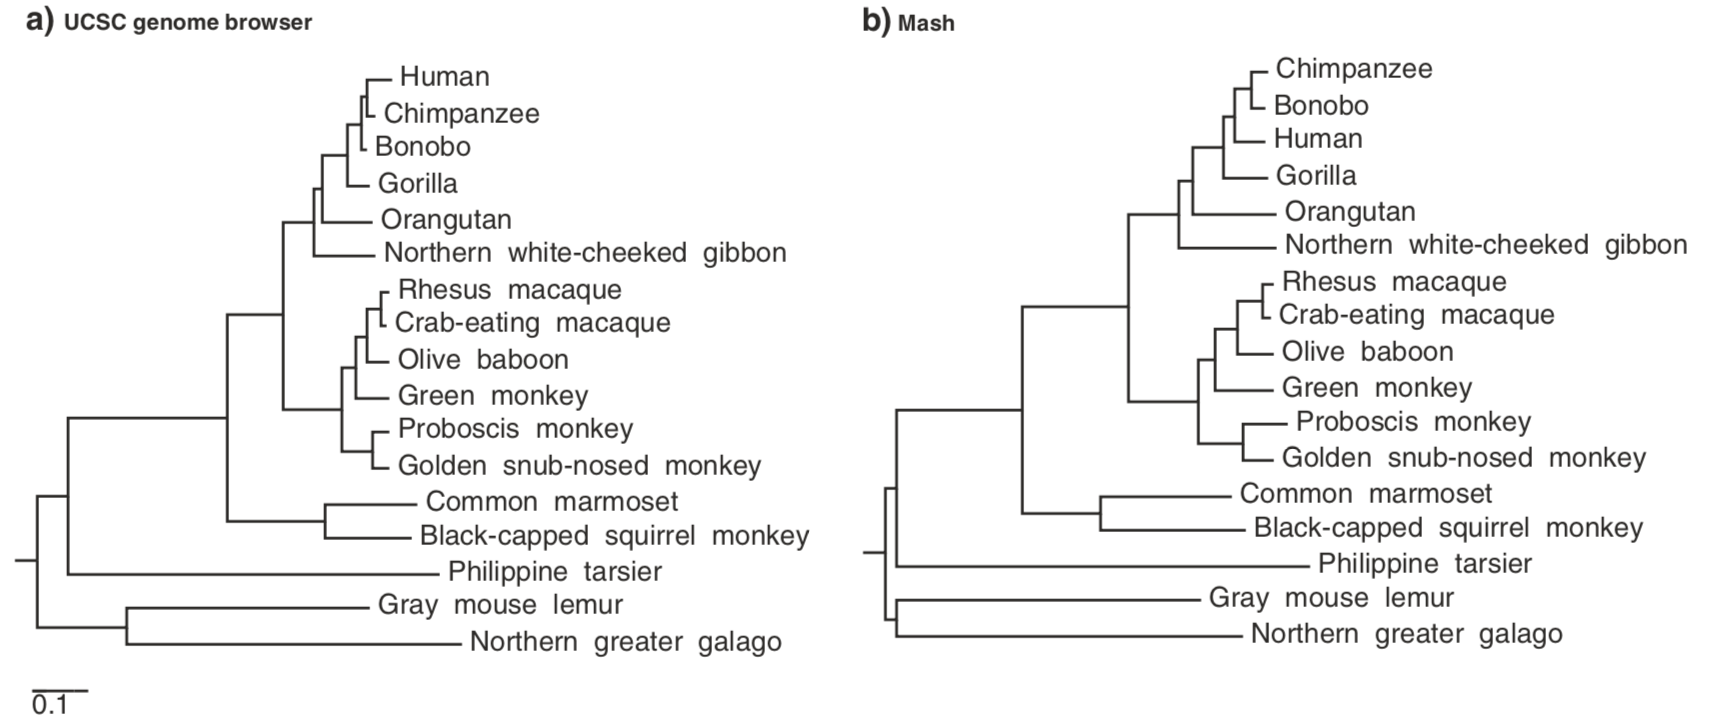
\includegraphics[width=1.0\textwidth]{Figure4_Ondov}
    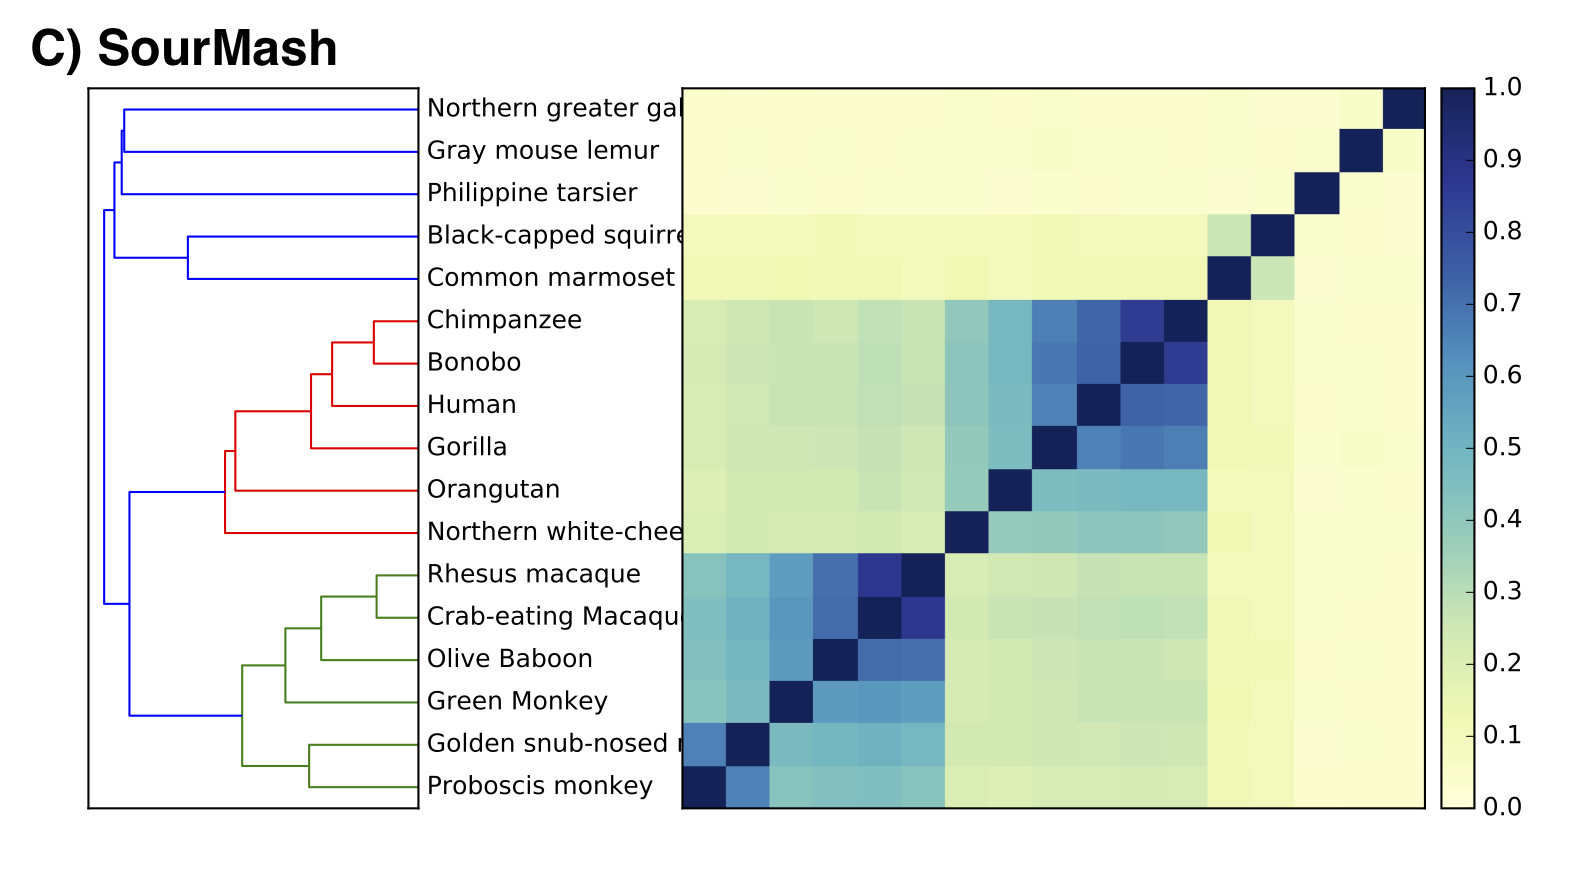
\includegraphics[width=1.0\textwidth]{Apes_Matrix_Common}
    \caption{A Comparison of Primate Phylogenetic Trees. \textbf{a} A primate phylogenetic tree model from the UCSC genome browser, with branch lengths derived from fourfold degenerate sites extracted from reference gene multiple alignments. \textbf{b} Ondov et al.'s Mash-based tree generated from whole genomes using a sketch size of s = 1000 and k-mer size of k = 21.\cite{MinHash} \textbf{c} SourMash-based tree generated from whole genomes using a sketch size of s = 1000 and k-mer size of k = 21.}
    \label{fig:Primate Tree}
\end{figure}
To evaluate MinHash on datasets with a high degree of similarity, we ran Minhash on over 300 E. Coli genomes downloaded from the NCBI Reference database. We were able to cluster E Coli strains and map similarities between strains.\ref{fig:All Ecoli} The minimum similarity within all genomes compared was a distance of 0.378 between Escherichia coli strain K-12 substrand MDS42 and Escherichia coli APEC O1. This is to be expected as a Multilocus sequence typing (MLST) of these two strains of E. coli yielded a similarity of only 98.1, far below the similarity with other E. coli strains.\cite{E coli}

\FloatBarrier
\begin{figure}[h]
    \centering
    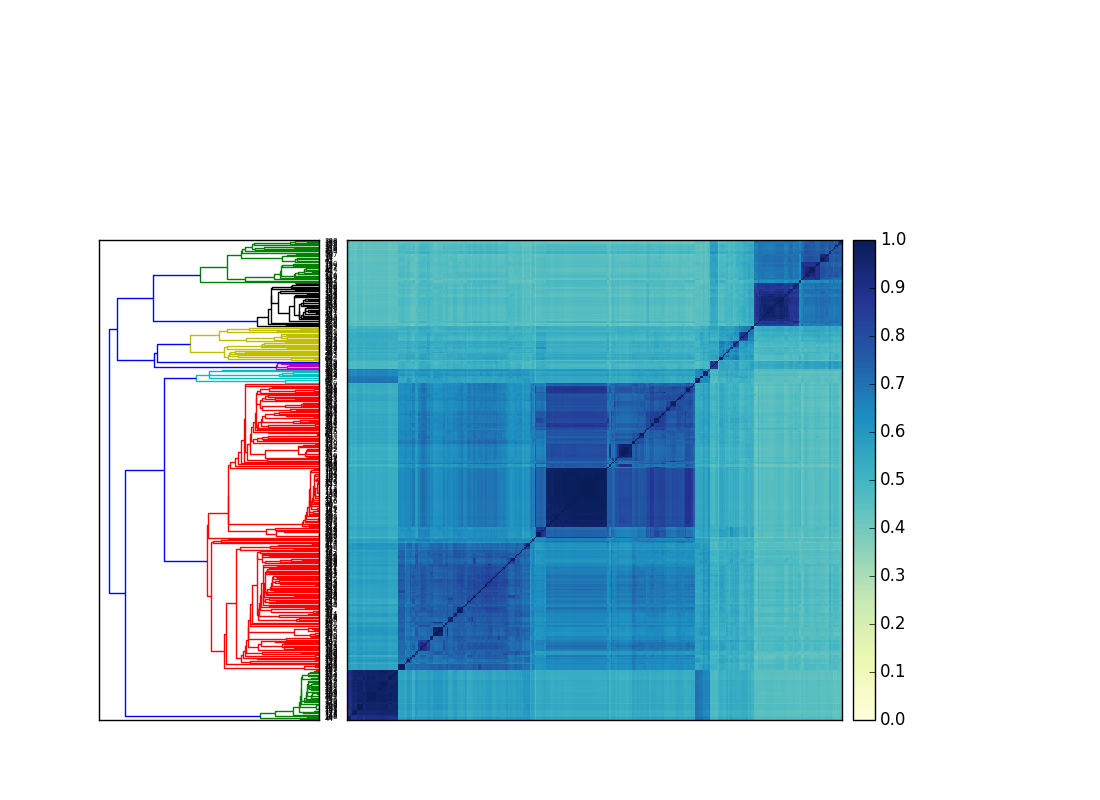
\includegraphics[width=1.0\textwidth]{All_E_coli}
    \caption{A Similarity Comparison of 397 \textit{E. coli} Species. This matrix shows similarity as darker in color. Note the darker colored diagonal line that stretches the matrix. This indicates the high similarity that occurs when a genome is compared to itself. The mminimum similarity within all genomes compared was a distance of 0.378 between Escherichia coli strain K-12 substrand MDS42 and Escherichia coli APEC O1.}
    \label{fig:All Ecoli}
\end{figure}
\FloatBarrier

\subsection{SimHash}
\FloatBarrier
\begin{figure}[h!]
	\centering
	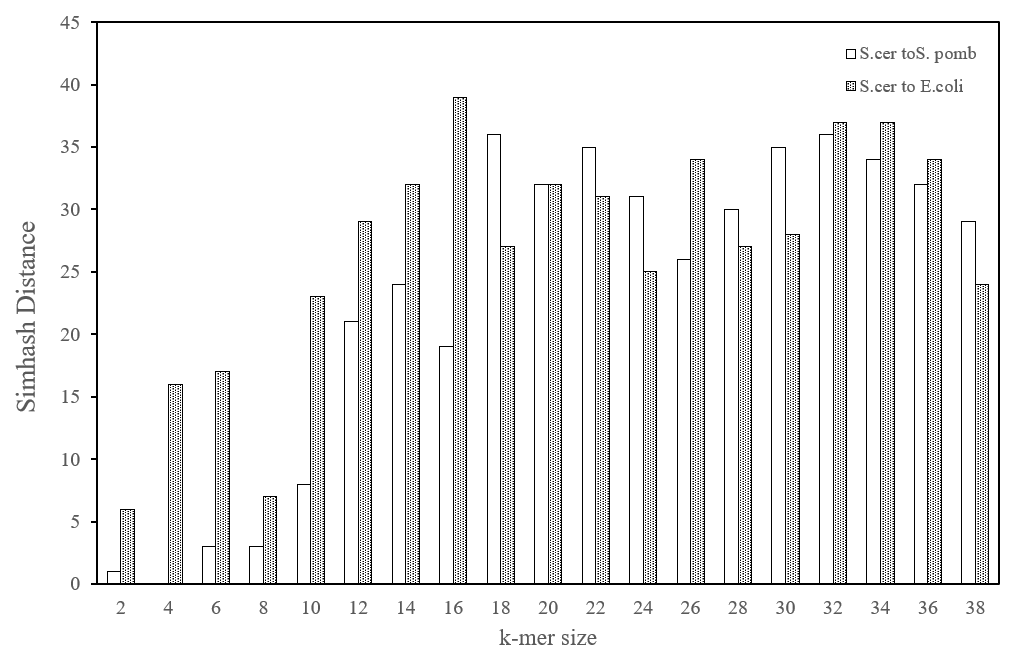
\includegraphics[width=1.0\textwidth]{Simhash_kmer_result.png}
	\caption{The S. cer, S. pomb and E. coli genomes have been inputted into the SimHash algorithm and the relative SimHash distances have been calculated pairwisely at the k-mer size from 2 to 38 at intervals of 2. As described in the methods section, the SimHash distance between S. cer and S. pomb is relative shorter than the one between S. cer to E. coli when the k-mer size is less than or equal to 16. However, as the k-mer size increases above 16, the SimHash algorithm fails to distinguish the relative distance between these 3 genomes.}
	\label{fig:SimHashDescription}
\end{figure}
\FloatBarrier


\subsection{SMASH}
\color{red} TO DO \color{black}
% ---------------------------------------------------------------------------------------------------------------------------
% Conclusions
% ---------------------------------------------------------------------------------------------------------------------------
\section{Conclusion}
Similarly to how MinHash needed to be adapted for genomic data processing with the culmination of the Mash algorithm, SimHash also needed to be adapted for genomic data processing with the culmination of the SMASH algorithm. Through the exploration and verification of Mash, followed by the exploration of SimHash and identification of the loss of resolution with respect to frequency of k-mers, to our development of the SMASH algorithm, we show that MinHash is not the only LSH that is applicable to the computational genomics field. Further refinement of the application of LSH into the computational genomics field would help increase performance not only with MinHash, but also with SimHash.


\section{Contributions of Each Member}
[1 paragraph] \color{red} TO DO \color{black}

% ---------------------------------------------------------------------------------------------------------------------------
% Bibliography
% ---------------------------------------------------------------------------------------------------------------------------
\begin{thebibliography}{9}

\bibitem{GitHub-SourMash} 
  C. Titus Brown and Luiz C. Irber, Jr.
  \textit{SourMash}.
  GitHub repository, https://github.com/dib-lab/sourmash, 2016.
  
\bibitem{E coli} 
  Timothy J. Johnson, Subhashinie Kariyawasam, Yvonne Wannemuehler, Paul Mangiamele, Sara J. Johnson, Curt Doetkott, Jerod A. Skyberg, Aaron M. Lynne, James R. Johnson, and Lisa K. Nolan.
  \textit{The Genome Sequence of Avian Pathogenic Escherichia coli Strain O1:K1:H7 Shares Strong Similarities with Human Extraintestinal Pathogenic E. coli Genomes}.
  Journal of Bacteriology, 189(8):3228-3236, 2007.
  
\bibitem{simhash} 
  Caitlin Sadowski and Greg Levin.
  \textit{SimHash: Hash-based Similarity Detection}.
  http://citeseerx.ist.psu.edu/viewdoc/download?doi=10.1.1.473.7179\&rep\\=rep1\&type=pdf, 
  2007.

\bibitem{SimvsMin} 
  Anshumali Shrivastava and Ping Li.
  \textit{In Defense of MinHash Over SimHash}.
  Journal of Machine Learning, 33, 2014.

\bibitem{MinHash} 
  Brian D. Ondov, Todd J. Treangen, Páll Melsted, Adam B. Mallonee, Nicholas H. Bergman, Sergey Koren and Adam M. Phillippy.
  \textit{Mash: fast genome and metagenome distance estimation using MinHash}.
  Genome Biology, 17:132, 2016.
  
\bibitem{Jellyfish}
  https://github.com/jamesturk/jellyfish

\bibitem{python-simhash}
  https://github.com/leonsim/simhash
  
\bibitem{go-simhash}  
  https://github.com/mfonda/simhash
  

\end{thebibliography}


\end{document}
